\documentclass{beamer}
\usepackage[utf8]{inputenc}
\usepackage[spanish]{babel}
\usepackage{graphicx}
\usepackage{hyperref}
\usepackage{amsmath}
\usepackage{amsthm}
\usepackage{amssymb}
\usepackage{subcaption}

\usetheme{Madrid}

% Draw
\usepackage{tikz}
\usetikzlibrary{positioning, arrows.meta, shapes.geometric, calc}
\tikzset{
  >={Stealth[length=3mm]},
  box/.style={draw, rounded corners, fill=blue!10, inner sep=6pt, text width=3cm, align=center, minimum height=3cm},
  data/.style={draw, ellipse, fill=green!10, inner sep=4pt, align=center},
}


% Code environment 
\usepackage{minted}
\usepackage{caption}

\setminted{
  mathescape,
  linenos,
  numbersep=3pt,
  frame=lines,
  framesep=1mm,
  baselinestretch=1,
  fontsize=\footnotesize,
  breaklines=true,
  xleftmargin=1em,
  xrightmargin=0em,
}

\newcommand{\codefile}[4][python]{%
  \captionsetup[listing]{name=Código}%
  \captionof{listing}{#2}%
  \label{#3}%
  \inputminted{#1}{#4}%
  }

% Pseudocode environment
\usepackage[ruled,vlined]{algorithm2e}
\renewcommand{\algorithmcfname}{Algoritmo}
\renewcommand{\algorithmautorefname}{Algoritmo}
\renewcommand{\listalgorithmcfname}{Índice de algoritmos}

% Environments
\usepackage{aliascnt}
\setbeamertemplate{theorems}[numbered]
\setbeamertemplate{theorem}[ams style]

\deftranslation[to=spanish]{Theorem}{Teorema}
\deftranslation[to=spanish]{Corollary}{Corolario}
\deftranslation[to=spanish]{Lemma}{Lema}
\deftranslation[to=spanish]{Proof}{Demostración}
\deftranslation[to=spanish]{Definition}{Definición}
\deftranslation[to=spanish]{Example}{Ejemplo}

% Commands 
\usepackage{xparse}
\usepackage[T1]{fontenc}
\usepackage{newtxmath}
\DeclareMathAlphabet{\mathpzc}{T1}{pzc}{m}{it}

\newcommand{\N}{\mathbb{N}}
\NewDocumentCommand{\R}{g g}{
  \IfNoValueTF{#1}
    {\mathbb{R}}
    {
    \IfNoValueTF{#2}
      {\mathbb{R}^{#1}}
      {\mathbb{R}^{#1 \times #2}}
    }
}
\newcommand{\E}{\mathcal{E}}
\newcommand{\K}{\mathcal{K}}
\newcommand{\M}{\mathcal{M}}
\newcommand{\C}{\mathcal{C}}
\newcommand{\A}{\mathcal{A}}
\newcommand{\B}{\mathcal{B}}
\newcommand{\X}{\mathcal{X}}
\newcommand{\Y}{\mathcal{Y}}
\newcommand{\nonce}{{\scriptstyle\mathpzc{N}}}
\newcommand{\Nonce}{\mathpzc{N}}


\graphicspath{{assets/}}

\title{Chosen Plaintext Attack (CPA)}
\subtitle{Una breve introducción con ejemplos prácticos}
\author[Emanuel N. Herrador]{Emanuel Nicolás Herrador}
\institute[FAMAF]{Facultad de Matemática, Astronomía, Física y Computación}
\date{Septiembre 2025}

\begin{document}
\frame{\titlepage}

\AtBeginSection[]{
  \begin{frame}
    \frametitle{Índice}
    \tableofcontents[currentsection]
  \end{frame}
}

\section{Motivación}
\begin{frame}{Motivación}
  Encriptación donde un tercero (\textit{atacante}) tiene acceso al oráculo de encriptación.
  I.e., puede dar múltiples mensajes y obtener sus correspondientes cifrados.
  \begin{example}
    Ana usando un servidor encriptando varios archivos con una misma key corta.
  \end{example}
  \begin{example}
    Comunicación no sincronizada entre Ana y Bob compartiendo una sola key en una red insegura.
  \end{example}
\end{frame}

\begin{frame}[allowframebreaks]{Idea}
  \begin{alertblock}{Tipo de cifrado}
    Si el cifrado es determinístico $\Rightarrow$ Es inseguro para este uso.
  \end{alertblock}
  Si es determinístico, entonces leakea información sobre el contenido porque se puede ver 
  fácilmente si dos mensajes son iguales.
  Además, deja abierto muchos ataques para obtener la key en base a los diferentes mensajes 
  cifrados de los plaintexts enviados por el atacante explotando alguna vulnerabilidad del 
  cifrado en sí o su implementación.
  \framebreak

  \begin{alertblock}{¿Qué usaremos?}
    Si queremos un cifrado que no sea vulnerable en este escenario, necesitaremos hacer uso 
    de \textit{cifrados probabilísticos}.
  \end{alertblock}
  De modo que diferentes encriptaciones de un mismo mensaje bajo la misma key (generalmente)
  producen diferentes ciphertexts.

  \begin{block}{Seguridad}
    La seguridad buscada en este escenario es \textit{semantic security against chosen
    plaintext attack}, o también conocida como \textit{CPA-security}.
  \end{block}
\end{frame}

\section{Contenido}
\begin{frame}{Contenido}
  Se hará un repaso de temas anteriores del libro: \textbf{semantic security} y \textbf{PRF}.

  Se presentarán, de forma general, los conceptos de \textbf{multi-key semantic security} y 
  \textbf{CPA-security}; junto con \textbf{construcciones de cifrados} CPA-secure
  (construcción genérica, randomized counter mode, CBC) junto con sus versiones \textbf{nonce-based}.

  En cuanto a ejemplos, se verán \textbf{vulnerabilidades en cifrados determinísticos} (AES ECB mode)
  y \textbf{mal uso del nonce} (AES CTR mode).
\end{frame}

\section{Repaso}
\begin{frame}[allowframebreaks]{Repaso}
  \begin{definition}[Semantic security game]
    Dados cifrado $\E = (E, D)$ definido sobre $(\K, \M, \C)$ y adversario $\A$, definimos dos 
    experimentos ($b = 0,1$) como:

    \begin{centering}
    \begin{tikzpicture}[node distance=50mm]
      \node[box] (chal) {Challenger (Experimento $b$) \\ $k \overset{\$}{\leftarrow} \K$ \\ $c \leftarrow E(k, m_b)$};
      \node[box, right=of chal] (adv1) {Adversario $\A$};

      \draw[->] ($(adv1.north west)+(0,-5mm)$) -- ($(chal.north east)+(0,-5mm)$) node[midway, above] {$m_0, m_1 \in \M : |m_0| = |m_1|$};
      \draw[->] (chal) -- (adv1) node[midway, above] {$c$};
      \draw[->] ($(adv1.south west)+(0,5mm)$) -- ($(chal.south east)+(0,5mm)$) node[midway, above] {$\hat{b} \in \{0, 1\}$};
    \end{tikzpicture}
    \end{centering}

    Sea $W_b$ el evento donde $\A$ envía $\hat{b} = 1$ en el Experimento $b$, la ventaja de $\A$
    sobre semantic security respecto a $\E$ es:
    \begin{equation*}
      \text{SSadv}[\A, \E] := \left|\text{Pr}[W_0] - \text{Pr}[W_1]\right|
    \end{equation*}
  \end{definition}

  \begin{definition}[Semantic security]
    $\E$ es semánticamente seguro si para todo adversario $\A$ eficiente, $\text{SSadv}[\A, \E]$
    es despreciable.
  \end{definition}

  \begin{alertblock}{Versión bit-guessing}
    Se considera el siguiente juego donde $\A$ gana si $\hat{b} = b$.

    \begin{centering}
    \begin{tikzpicture}[node distance=50mm]
      \node[box] (chal) {Challenger \\ $b \overset{\$}{\leftarrow} \{0, 1\}$ \\ $k \overset{\$}{\leftarrow} \K$ \\ $c \leftarrow E(k, m_b)$};
      \node[box, right=of chal] (adv1) {Adversario $\A$};

      \draw[->] ($(adv1.north west)+(0,-5mm)$) -- ($(chal.north east)+(0,-5mm)$) node[midway, above] {$m_0, m_1 \in \M : |m_0| = |m_1|$};
      \draw[->] (chal) -- (adv1) node[midway, above] {$c$};
      \draw[->] ($(adv1.south west)+(0,5mm)$) -- ($(chal.south east)+(0,5mm)$) node[midway, above] {$\hat{b} \in \{0, 1\}$};
    \end{tikzpicture}
    \end{centering}

    Donde si el evento $W$ es cuando $\A$ gana, la ventaja es:
    \begin{equation*}
      \text{SSadv}^*[\A, \E] = \left|\text{Pr}[W] - \frac{1}{2}\right|
    \end{equation*}
    Se cumple que $\text{SSadv}[\A, \E] = 2 \cdot \text{SSadv}^*[\A, \E]$.
  \end{alertblock}

  \begin{block}{Idea sobre PRF}
    Sean $\K, \X, \Y$ conjuntos finitos y $F : \K \times \X \to \Y$, se pretende que $F$ sea un 
    algoritmo determinista eficiente y tal que $F(k, \cdot)$ \textit{luzca} como una 
    función random $\X \to \Y$.

    Es decir, que $F(k, \cdot)$ parezca elegida uniformemente del conjunto $\text{Funs}[\X, \Y]$
    de todas las funciones $f : \X \to \Y$.
  \end{block}
  \begin{block}{Idea sobre seguridad de PRF}
    Sigue el mismo esquema que el anterior solo que los adversarios tienen $Q$ queries antes 
    de tener que adivinar el tipo de experimento (si viene de $F$ o de $\text{Funs}[\X, \Y]$).

    La ventaja se define de la misma forma, al igual que los PRFs seguros y su versión 
    bit-guessing.
  \end{block}
\end{frame}

\section{Multi-key attacks}
\begin{frame}[allowframebreaks]{Multi-key attacks}
  Dado un cifrado semánticamente seguro, ¿puedo usarlo para cifrar más de un mensaje tomando 
  claves diferentes para cada uno?

  \begin{definition}[Multi-key semantic security]
    Dado cifrado $\E = (E, D)$ definido sobre $(\K, \M, \C)$ y adversario $\A$, definimos los 
    experimentos $b = 0,1$ (con $q$ queries) como:

    \begin{centering}
    \begin{tikzpicture}[node distance=50mm]
      \node[box] (chal) {Challenger (Experimento $b$) \\ $k_i \overset{\$}{\leftarrow} \K$ \\ $c_i \leftarrow E(k_i, m_{ib})$};
      \node[box, right=of chal] (adv1) {Adversario $\A$};

      \draw[->] ($(adv1.north west)+(0,-5mm)$) -- ($(chal.north east)+(0,-5mm)$) node[midway, above] {$m_{i0}, m_{i1} \in \M : |m_{i0}| = |m_{i1}|$};
      \draw[->] ($(chal.north east)+(0,-11mm)$) -- ($(adv1.north west)+(0,-11mm)$) node[midway, above] {$c_i$};
      \node at ($(chal)!0.5!(adv1)+(0,1mm)$) {$\vdots$};
      \draw[->] ($(adv1.south west)+(0,5mm)$) -- ($(chal.south east)+(0,5mm)$) node[midway, above] {$\hat{b} \in \{0, 1\}$};
    \end{tikzpicture}
    \end{centering}

    La ventaja es
    \begin{equation*}
      \text{MSSadv}[\A, \E] := \left|\text{Pr}[W_0] - \text{Pr}[W_1]\right|
    \end{equation*}
    y $\E$ es semánticamente seguro para múltiples claves si para todo adversario $\A$ la ventaja 
    es despreciable.
  \end{definition}

  \begin{theorem}
    Si $\E$ es semánticamente seguro, entonces es también semánticamente seguro para múltiples claves.

    I.e., semantic security $\Rightarrow$ multi-key semantic security.
  \end{theorem}
  \begin{proof}
    Supongamos el juego visto antes para multi-key security.
    Como $\E$ es semánticamente seguro, entonces si para $i \overset{\$}{\leftarrow} \{1, \dots, k\}$ 
    modifico el Challenger para que encripte $m_{i\bar{b}}$ en vez de $m_{ib}$ (donde
    $\bar{b}$ es el complemento de $b$ en $\{0, 1\}$), entonces $\A$ no puede notar la
    diferencia.
    Siguiendo el argumento para las $Q$ queries, cambiamos todo el experimento completo.
    Luego, $\A$ no puede distinguir tampoco el juego multi-key.
  \end{proof}
\end{frame}

\section{Semantic security against chosen plaintext attack}
\begin{frame}[allowframebreaks]{CPA security}
  \begin{definition}[CPA security]
    Dados $\E = (E, D)$ definido sobre $(\K, \M, \C)$ y adversario $\A$, definimos los 
    experimentos $b = 0,1$ con queries como:

    \begin{centering}
    \begin{tikzpicture}[node distance=50mm]
      \node[box] (chal) {Challenger (Experimento $b$) \\ $k \overset{\$}{\leftarrow} \K$ \\ $c_i \leftarrow E(k, m_{ib})$};
      \node[box, right=of chal] (adv1) {Adversario $\A$};

      \draw[->] ($(adv1.north west)+(0,-5mm)$) -- ($(chal.north east)+(0,-5mm)$) node[midway, above] {$m_{i0}, m_{i1} \in \M : |m_{i0}| = |m_{i1}|$};
      \draw[->] ($(chal.north east)+(0,-11mm)$) -- ($(adv1.north west)+(0,-11mm)$) node[midway, above] {$c_i$};
      \node at ($(chal)!0.5!(adv1)+(0,1mm)$) {$\vdots$};
      \draw[->] ($(adv1.south west)+(0,5mm)$) -- ($(chal.south east)+(0,5mm)$) node[midway, above] {$\hat{b} \in \{0, 1\}$};
    \end{tikzpicture}
    \end{centering}

    Donde la ventaja es:
    \begin{equation*}
      \text{CPAadv}[\A, \E] := \left|\text{Pr}[W_0] - \text{Pr}[W_1]\right|
    \end{equation*}
    Y $\E$ es \textit{CPA secure} si $\forall \A$ adversario eficiente, su ventaja 
    es despreciable.
  \end{definition}

  \begin{block}{Nota}
    El juego es el mismo que para multi-key semantic security solo que se usa una sola 
    key $k$.

    Tiene la variante bit-guessing donde $\text{CPAadv}^*[\A, \E] := \left|\text{Pr}[\hat{b} = b] - \frac{1}{2}\right|$
    y $\text{CPAadv}^*[\A, \E] = 2 \cdot \text{CPAadv}^*[\A, \E]$.

    Se suele llamar también como \textbf{IND-CPA} (indistinguishable against chosen plaintexts 
    attacks) porque el juego sobre el que se define este concepto de seguridad se basa 
    en no poder distinguir de qué mensaje viene el ciphertext.
    Es decir, que parezca uniformemente distribuido en $\C$.
  \end{block}
\end{frame}

\section{Vulnerabilidad de ciphers determinísticos}
\begin{frame}{Casos sencillos}
  Algunos ejemplos de cifrados vulnerables ante CPA son \textit{caesar cipher},
  \textit{Vignère} o \textit{XOR simple} con misma key.

  Uno más complejo es \textit{RC4} cuando se reutiliza la misma clave $k$ para varios 
  mensajes (debido a que se repite el keystream), dado que se puede recuperar todo 
  el keystream.
  Sin embargo, el caso donde no se repite sigue siendo inseguro porque $\A$ puede enviar 
  varios plaintexts y observar los correspondientes ciphertexts para recuperar parcialmente 
  la key debido a que los primeros bytes del keystream generado están sesgados (no son del 
  todo aleatorios).
\end{frame}

\begin{frame}[allowframebreaks, fragile]{ECB vs. CBC}
  Considerando el cifrado por bloques AES, el modo ECB es determinístico mientras que CBC probabilístico.
  Podemos ver el leakage de ECB en el ejemplo de encriptar una imagen:
  \begin{figure}[h!]
    \centering 
    \begin{subfigure}[b]{0.3\textwidth}
      \centering 
      
\includegraphics[width=\textwidth]{Tux.png}
      \caption{Imagen original}
    \end{subfigure}
    \hfill
    \begin{subfigure}[b]{0.3\textwidth}
      \centering 
      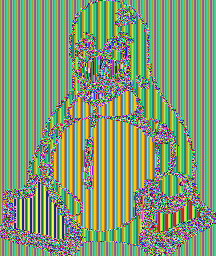
\includegraphics[width=\textwidth]{Tux-ecb.png}
      \caption{Modo ECB}
    \end{subfigure}
    \hfill
    \begin{subfigure}[b]{0.3\textwidth}
      \centering 
      
\includegraphics[width=\textwidth]{Tux-cbc.png}
      \caption{Modo CBC}
    \end{subfigure}
  \end{figure}

  \begin{alertblock}{¿Cómo obtener estas imágenes?}
    El código es análogo tanto para ECB como para CBC:
    \begin{minted}[fontsize=\small]{bash}
magick Tux.svg Tux.ppm 
head -n 3 Tux.ppm > header.txt 
tail -n +4 Tux.ppm > body.bin 
openssl enc -aes-128-ecb -nosalt -pass pass:"password" -in body.bin -out body.ecb.bin 
cat header.txt body.enc.bin > Tux.ecb.ppm 
magick Tux.ecb.ppm Tux-ecb.svg
    \end{minted}
  \end{alertblock}

  \begin{example}{Demo}
    CTF challenge de CryptoHack: \href{https://aes.cryptohack.org/ecb_oracle/}{ECB Oracle}.
  \end{example}
\end{frame}

\section{Construcción de cifrados CPA secure}
\begin{frame}[allowframebreaks]{Construcción genérica}
  Veremos cómo convertir cualquier cifrado semánticamente seguro $\E = (E, D)$ en un cifrado 
  $\E'$ CPA secure usando una PRF $F$ adecuada.
  \begin{block}{Construcción}
    Sea $\E = (E, D)$ definido sobre $(\K, \M, \C)$ y $F$ una PRF definida sobre $(\K', \X, \K)$,
    definimos $\E' = (E', D')$ definido sobre $(\K', \M, \X \times \C)$ como:
    \begin{figure}[h]
      \centering
      \begin{minipage}{0.48\textwidth}
        \begin{algorithm}[H]
          \DontPrintSemicolon
          \footnotesize
          \caption{$E'(k', m)$}
          \KwIn{$k' \in \K',\ m \in \M$}
          \KwOut{$(x, c) \in \X \times \C$}
          $x \overset{\$}{\leftarrow} \X$\;
          $k \leftarrow F(k',x)$\;
          $c \leftarrow E(k, m)$\;
          \KwRet{$(x, c)$}
        \end{algorithm}
      \end{minipage}
      \hfill
      \begin{minipage}{0.48\textwidth}
        \begin{algorithm}[H]
          \DontPrintSemicolon
          \footnotesize
          \caption{$D'(k', c')$}
          \KwIn{$k' \in \K, c' = (x,c) \in \X \times \C$}
          \KwOut{$m \in \M$}
          $k \leftarrow F(k', x)$\;
          $m \leftarrow D(k, c)$\;
          \KwRet{$m$}
        \end{algorithm}
      \end{minipage}
    \end{figure}
  \end{block}

  \begin{theorem}
    Si $F$ es una PRF segura, $\E$ un cifrado semánticamente seguro y $N := |\X|$ \textit{super-poly}
    (i.e., tal que $\frac{1}{N}$ es despreciable), entonces el cifrado $\E'$ definido anteriormente 
    es CPA seguro.

    Además, sea $\A$ el adversario que ataca a $\E'$, su ventaja cumple que:
    \begin{equation*}
      \text{CPAadv}[\A, \E'] \leq \frac{Q^2}{N} + 2 \cdot \text{PRFadv}[\B_F, F] + Q \cdot \text{SSadv}[\B_\E, \E]
    \end{equation*}
    donde se considera el juego de CPA-security con $Q$ queries, y tal que existen los 
    adversarios $\B_F$ que ataca al juego de PRF security, y $\B_\E$ para el de semantic security.
    $\B_F, \B_\E$ son elementos del adversario $\A$.
  \end{theorem}
  \begin{block}{Nota}
    Se pide que $\frac{1}{N}$ sea despreciable para que la probabilidad de que $F$ genere el mismo 
    valor $x$ dos veces sea despreciable.
  \end{block}
  \begin{proof}[Idea de la demostración]
    Como $F$ es una PRF segura, entonces podemos reemplazar $F$ como una verdadera función random.
    Usando la suposición de que $N$ es super-poly, entonces la probabilidad de que dos valores
    $x \in \X$ generados sean el mismo, es despreciable.
    Luego, en este escenario eso significa que las claves del challenger son todas generadas 
    de forma independiente.
    Finalmente, el juego se reduce al de multi-key security.
    Por ello, por teorema como $\E$ es semánticamente seguro, también es semánticamente seguro 
    para claves múltiples.
    Esto se puede extender a $\E'$.
  \end{proof}
\end{frame}

\begin{frame}[allowframebreaks]{Randomized counter mode}
  \begin{block}{Construcción}
    Sea $F: \K \times \X \to \Y$ una PRF con $\X = \{0, \dots, N-1\},\ \Y = \{0, 1\}^n$.
    Para cualquier $\ell \geq 1$ acotado polinómicamente, definimos el cifrado $\E = (E, D)$
    sobre $(\K, \Y^{\leq\ell}, \X \times \Y^{\leq\ell})$ como:
    \begin{figure}[h]
      \centering
      \begin{minipage}{0.48\textwidth}
        \begin{algorithm}[H]
          \DontPrintSemicolon
          \footnotesize
          \caption{$E(k, m)$}
          \KwIn{$k \in \K, m \in \Y^{\leq\ell} : v := |m|$}
          \KwOut{$(x, c) \in \X \times \Y^v$}
          $x \overset{\$}{\leftarrow} \X$\;
          \For{$j \leftarrow 0$ \textbf{to} $v-1$}{
            $c[j] \leftarrow F(k, x + j \mod N) \oplus m[j]$\;
          }
          \KwRet{$(x, c)$}
        \end{algorithm}
      \end{minipage}
      \hfill
      \begin{minipage}{0.48\textwidth}
        \begin{algorithm}[H]
          \DontPrintSemicolon
          \footnotesize
          \caption{$D(k, c')$}
          \KwIn{$k \in \K, c' = (x, c) \in \X \times \Y^{\leq\ell} : v := |c|$}
          \KwOut{$m \in \Y^v$}
          \For{$j \leftarrow 0$ \textbf{to} $v-1$}{
            $m[j] \leftarrow F(k, x + j \mod N) \oplus c[j]$\;
          }
          \KwRet{$m$}
        \end{algorithm}
      \end{minipage}
    \end{figure}
  \end{block}
  La componente $x$ del ciphertext es llamada típicamente como \textit{valor inicial} 
  o $\textbf{IV}$.

  \begin{theorem}
    Si $F$ es una PRF segura y $N$ super-poly, entonces para cualquier $\ell \geq 1$ acotado 
    polinómicamente, el cifrado $\E$ definido anteriormente es CPA seguro.

    Además, sea $\A$ el adversario que ataca a $\E'$ en el juego de CPA-security con
    $Q$ queries, su ventaja cumple que:
    \begin{equation*}
      \text{CPAadv}[\A, \E] \leq \frac{2Q^2\ell}{N} + 2 \cdot \text{PRFadv}[\B,F]
    \end{equation*}
    donde $\B$ es el adversario que ataca a $F$ en el juego de PRF security y es un 
    elemento de $\A$.
  \end{theorem}
  \begin{proof}[Idea de la demostración]
    Como $F$ es PRF segura, podemos reemplazarla por una función random $f$.
    Como $N$ es super-poly y cada IV es elegido random, entonces el challenger nunca evalúa 
    $f$ en el mismo punto dos veces, excepto con probabilidad despreciable.
    En este escenario, significa que la encriptación de cada mensaje es un OTP independiente.
    Luego, la ventaja de $\A$ en CPA-security game es despreciable.
  \end{proof}
\end{frame}

\begin{frame}[allowframebreaks]{Modo CBC}
  Como ejemplo de un cifrado por bloques CPA seguro:
  \begin{block}{Construcción}
    Dados $\E = (E, D)$ un cifrado por bloques definido sobre $(\K, \X)$ donde $\X = \{0, 1\}^n$;
    $N := |\X| = 2^n$ y $\ell \geq 1$ acotado polinómicamente, entonces definimos el cifrado 
    $\E' = (E', D')$ sobre $(\K, \X^{\leq\ell}, \X^{\leq\ell + 1}\setminus\X^0)$ como:
    \begin{figure}[h]
      \centering
      \begin{minipage}{0.48\textwidth}
        \begin{algorithm}[H]
          \DontPrintSemicolon
          \footnotesize
          \caption{$E'(k, m)$}
          \KwIn{$k \in \K, m \in \X^{\leq\ell} : v := |m|$}
          \KwOut{$c \in \X^{\leq\ell + 1}\setminus\X^0$}
          $c[0] \overset{\$}{\leftarrow} \X$\;
          \For{$j \leftarrow 0$ \textbf{to} $v-1$}{
            $c[j+1] \leftarrow E(k, c[j] \oplus m[j])$\;
          }
          \KwRet{$c$}
        \end{algorithm}
      \end{minipage}
      \hfill
      \begin{minipage}{0.48\textwidth}
        \begin{algorithm}[H]
          \DontPrintSemicolon
          \footnotesize
          \caption{$D'(k, c)$}
          \KwIn{$k \in \K, c \in \X^{\leq\ell+1\setminus\X^0} : v := |c|-1$}
          \KwOut{$m \in \X^v$}
          \For{$j \leftarrow 0$ \textbf{to} $v-1$}{
            $m[j] \leftarrow D(k, c[j+1]) \oplus c[j]$\;
          }
          \KwRet{$m$}
        \end{algorithm}
      \end{minipage}
    \end{figure}
  \end{block}

  Aquí, la primer componente $c[0]$ es el IV.
  \begin{theorem}
    Si $\E = (E, D)$ es un cifrado seguro por bloques definido sobre $(\K, \X)$ y $N := |\X|$
    es super-poly, entonces para cualquier $\ell\geq 1$ acotado polinómicamente, el cifrado 
    $\E'$ definido anteriormente es CPA seguro.

    Sea $\A$ el adversario para CPA de $\E'$ con $Q$ queries, su ventaja cumple:
    \begin{equation*}
      \text{CPAadv}[\A, \E'] \leq \frac{2Q^2\ell^2}{N} + 2 \cdot \text{BCadv}[\B, \E]
    \end{equation*}
    donde $\B$ es el adversario que ataca a $\E$ en el juego de seguridad de cifrados por bloques,
    y que forma parte de $\A$.
  \end{theorem}
  \begin{proof}
    La prueba es análoga a la anterior porque por corolario de \textbf{PRF Switching Lemma},
    $\E = (E, D)$ cifrado por bloques definido sobre $(\K, \X)$ con $N := |\X|$ super-poly
    es un cifrado por bloques seguro si y solo si $E$ es una PRF segura.
  \end{proof}
  \begin{block}{Nota}
    No agrego PRF Switching Lemma como contenido de repaso o adicional porque requiere 
    agregar también las nociones de concepto de cifrado por bloques y su seguridad.
  \end{block}
\end{frame}

\section{Nonce-based encryption}
\begin{frame}[allowframebreaks]{Encriptación nonce-based}
  Todos los esquemas de cifrado vistos sufren de \textit{expansión del ciphertext}, es decir,
  los mensajes cifrados son más largos que los originales.
  Para ello, la idea es agregar un input más $\nonce$ a los algoritmos de encriptación y 
  decriptación; convirtiendo a estos ahora en determinísticos.

  La intención es que un mensaje encriptado con un nonce debe ser desencriptado con el mismo 
  nonce.
  \begin{block}{Correctitud}
    $\forall k \in \K, m \in \M, \nonce \in \Nonce,\ D(k, E(k, m, \nonce), \nonce) = m$.
  \end{block}

  \begin{definition}[nonce-based CPA security]
    Dados cifrado $\E = (E, D)$ definido sobre $(\K, \M, \C, \Nonce)$, y adversario $\A$,
    se definen los experimentos $b = 0,1$ como:

    \begin{centering}
    \begin{tikzpicture}[node distance=50mm]
      \node[box] (chal) {
        Challenger (Experimento $b$) \\
        $k \overset{\$}{\leftarrow} \K$ \\
        $c_i \leftarrow E(k, m_{ib}, \nonce_i)$
      };
      \node[box, right=of chal] (adv1) {Adversario $\A$};

      \draw[->]
        ($(adv1.north west)+(0,-5mm)$) -- ($(chal.north east)+(0,-5mm)$)
        node[midway, above] {
          $\begin{aligned}
            m_{i0}, m_{i1} &\in \M : |m_{i0}| = |m_{i1}|\\ 
            \nonce_i &\in \Nonce\setminus\{\nonce_1,\dots,\nonce_{i-1}\}
          \end{aligned}$
        };
      \draw[->]
        ($(chal.north east)+(0,-11mm)$) -- ($(adv1.north west)+(0,-11mm)$)
        node[midway, above] {$c_i$};
      \node at ($(chal)!0.5!(adv1)+(0,1mm)$) {$\vdots$};
      \draw[->]
        ($(adv1.south west)+(0,5mm)$) -- ($(chal.south east)+(0,5mm)$)
        node[midway, above] {$\hat{b} \in \{0, 1\}$};
    \end{tikzpicture}
    \end{centering}

    La ventaja se define como:
    \begin{equation*}
      \text{nCPAadv}[\A, \E] := \left|\text{Pr}[W_0] - \text{Pr}[W_1]\right|
    \end{equation*}
  \end{definition}

  \begin{block}{Nota}
    La ventaja se define asumiendo que ningún nonce es usado más de una vez en el proceso 
    de encriptación.

    También se define su versión bit-guessing con
    \begin{equation*}
      \text{nCPAadv}[\A, \E] = 2 \cdot \text{nCPAadv}^*[\A, \E]
    \end{equation*}
    donde $\text{nCPAadv}^*[\A,\E] := \left|\text{Pr}[\hat{b} = b] - \frac{1}{2}\right|$
  \end{block}
  \begin{definition}[nonce-based CPA security]
    Un cifrado $\E$ nonce-based es CPA seguro si para todo adversario eficiente $\A$, la ventaja 
    $\text{nCPAadv}[\A, \E]$ es despreciable.
  \end{definition}
\end{frame}

\begin{frame}[allowframebreaks]{Modificaciones a ciphers CPA-secure para ser nonce-based}
  \begin{block}{Cifrado genérico nonce-based}
    Se debe tratar el valor $x \in \X$ como un nonce.
  \end{block}
  \begin{block}{Nonce-based counter mode}
    Asumiendo que $\ell | N$ (en la práctica son potencias de $2$), $\Nonce = \{0,\dots,\frac{N}{\ell}-1\}$
    y el input a la PRF $F$ debe ser $x := \nonce\ell$.
    De este modo, $\nonce_1 \neq \nonce_2 \in \Nonce \Rightarrow \{x_1,\dots,x_1+\ell-1\} \cap \{x_2,\dots,x_2+\ell-1\} = \emptyset$
    para $x_1 := \nonce_1\ell,\ x_2 := \nonce_2\ell$.
  \end{block}
  \begin{block}{Nonce-based CBC mode}
    La idea es mapear nonce a pseudorandom IV usando una PRF sobre $(\K',\Nonce,\X)$ con 
    $\K', \Nonce$ arbitrarios.
    De este modo, sea $\E'$ este cifrado, el espacio de claves es $\K \times \K'$ y el 
    IV se computa como $c[0] := F(k', \nonce)$.
  \end{block}
  \begin{block}{CPA-security}
    Todos son CPA seguros bajo condición de que sus elementos (PRFs, cifrado por bloques) 
    también sean seguros, así como también se mantienen las variables acotadas polinómicamente
    y los super-poly.
  \end{block}
\end{frame}
\begin{frame}{Vulnerabilidades ante mal uso de nonces}
  \begin{example}
    Demo CTF challenge de la Hacker Class COMPFEST16: \textit{Reduce, Reuse, Recycle}
  \end{example}
\end{frame}

\begin{frame}
  \centering 
  \vfill 
  {\Huge \textbf{¡Gracias!}}
  \vfill
\end{frame}

\end{document}
